\chapter{Automatic generator}
The automatic generator of Gr\"obner basis solvers is used to easily solve problems leading to systems of polynomial equations. These systems usually arise when solving minimal problems \cite{MinimalProblems} in computer vision. Typically, these systems are not trivial so special solvers have to be designed for concrete problems to achieve efficient and numerically stable solvers. But solvers generated for concrete problems can not be easily applied for similar or new problems and therefore the automatic generator was proposed in \cite{AutoGen}. Solvers generated by the automatic generator can be easily used to solve complex problems even by non-experts users.

The input of the automatic generator is a system of polynomial equations with a finite number of solutions and the output is a MATLAB or a Maple code that computes solutions of the given system for arbitary coefficients. One of the goals of this thesis is to improve previous implementation \cite{AutoGen} of the automatic generator to construct more efficient and numerically stable solvers.

The newest version of the automatic genenerator implemented in MATLAB can be downloaded from \cite{AutomaticGenerator}.

\section{Description of the automatic generator}
In this section we would like to briefly describe the procedure for generating solvers. The automatic generator consists of several independent modules, see Figure \ref{autogen:blockDiagram}. Since all these modules are independent, they can be easily improved or replaced by more efficient implementations. Next we describe each of these modules, full description can be found in \cite{AutoGen}.

\begin{figure}[ht]
  \centering
  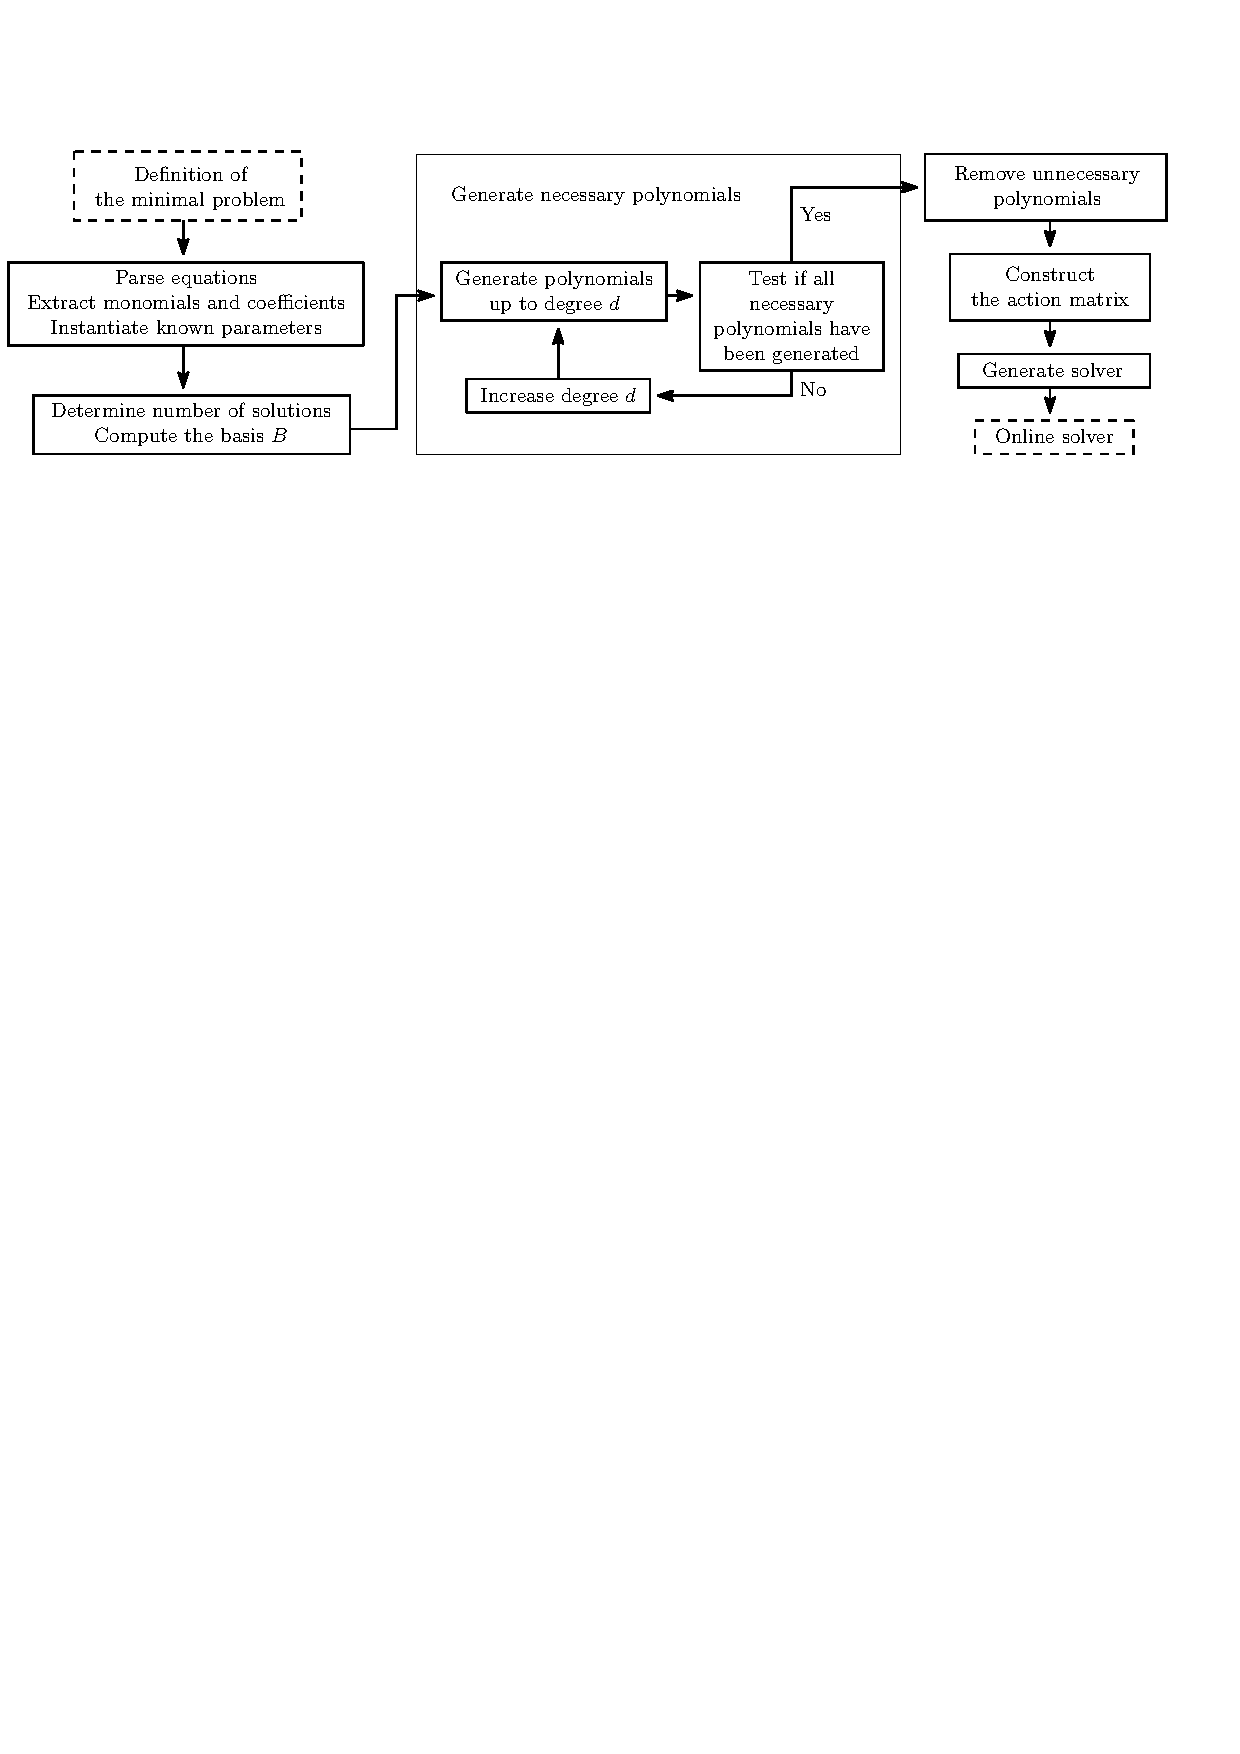
\includegraphics[width=0.95\textwidth]{AutomaticGenerator.pdf}
  \caption{Block diagram of the automatic generator}
  \label{autogen:blockDiagram}
\end{figure}

\subsection{Definition of the minimal problem}
Definitions of minimal problems are written in separate functions that are stored in the folder \texttt{minimalProblems}. Each of the definitions has to contain few necessary information about the minimal problem. First of all, the system of polynomial equations with symbolic variables and parameters has to be provided. Next we have to specify the list of unknown variables and known parameters. Optionally if we know the monomial basis $B$ of the polynomial system in advance we can specify it to save some computation time. The monomial basis $B$ is a set $\left\{m\ |\ \overline{m}^G = m\right\}$ where $m$ is a monomial and $G$ is the Gr\"obner basis of the given polynomial system. At last we have to set some settings for the automatic generator. We recommend to obtain the default settings by calling the function \textit{gbs\_InitConfig()} and only overwrite the settings we want to change. In the folder \texttt{minimalProblem} there are some examples which are self explanatory and can be used as templates to create new minimal problem definitions.

\subsection{Equations parser, Instantiating}
In the next step we have to parse the given equations, that means we extract used monomials and parameters and obtain total degrees of the polynomials. Then we instantiate each known parameter with a random number from $\mathbb{Z}_p$. We assign unique identifier to each used parameter. The reason is that we need to track the parameters through the process of adding polynomials in order to be able to restore the process in the solver generation module.

\section{Reimplementation}

\section{Multiple eliminations solver}

\section{Removing unnecessary polynomials}

\section{Matrix partitioning}

\section{F4 strategy}
